\chapter{Relative and Composite Motion}
\label{ch:relative}
\begin{chapterintro}
\textbf{You will learn to:} transform velocities and accelerations between
reference frames; use the composition laws; analyse motion in a rotating frame;
and identify the Coriolis and centrifugal terms.
\end{chapterintro}

\section{Galilean transformation}

Let $R(O,x,y,z)$ be a fixed frame and $R'(O',x',y',z')$ a frame moving with
constant velocity $\vec V$ relative to $R$, without rotation. Then
\[
\vec r=\vec r'+\vec Vt,\qquad
\vec v=\vec v'+\vec V,\qquad
\vec a=\vec a'.
\]
The acceleration is the same in both frames. Such frames are \textbf{inertial}:
Newton's laws have the same form in all of them. This is Galilean relativity.

\section{Composition of velocities and accelerations}

For a general moving frame (translating and rotating), let
\begin{itemize}[leftmargin=1.4em,itemsep=2pt]
  \item $\vec v_a$ be the absolute velocity (relative to $R$);
  \item $\vec v_r$ the relative velocity (relative to $R'$);
  \item $\vec v_e$ the entrainment (drag) velocity, i.e.\ the velocity in $R$ of
        the point of $R'$ coinciding with $M$.
\end{itemize}
Then
\[
\boxed{\vec v_a=\vec v_r+\vec v_e.}
\]
For a frame rotating with angular velocity $\vec\Omega$,
\[
\vec v_e=\vec v(O'/R)+\vec\Omega\times\vec{O'M}.
\]
The acceleration composition law is
\[
\boxed{\vec a_a=\vec a_r+\vec a_e+\vec a_c,}
\]
where
\[
\vec a_e=\vec a(O'/R)+\frac{\dd\vec\Omega}{\dd t}\times\vec{O'M}
+\vec\Omega\times\left(\vec\Omega\times\vec{O'M}\right),
\]
and the \textbf{Coriolis acceleration} is
\[
\vec a_c=2\vec\Omega\times\vec v_r.
\]

\begin{figure}[htbp]
\centering
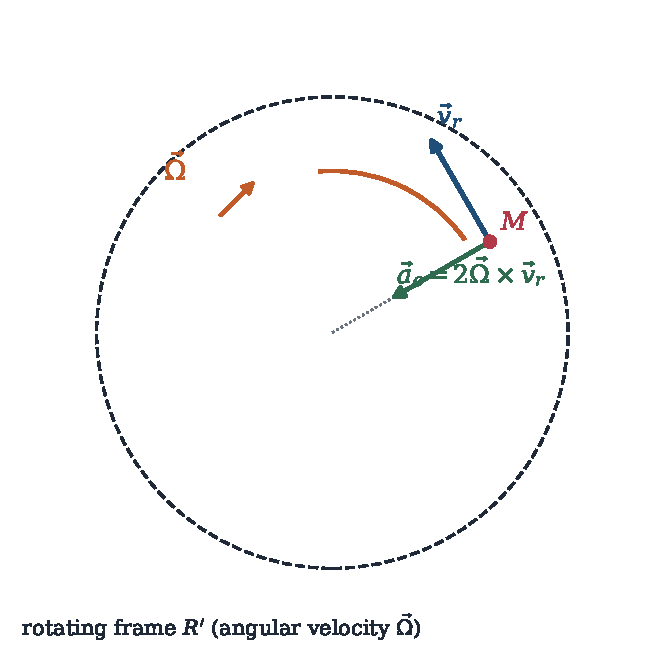
\includegraphics[width=0.72\textwidth]{figures/10_rotating_frame.pdf}
\caption{A point $M$ moving in a rotating frame. The Coriolis acceleration is
perpendicular to both the angular velocity and the relative velocity.}
\label{fig:rotating-frame}
\end{figure}

\section{Non-inertial frames and fictitious forces}

Newton's second law in an inertial frame is $m\vec a_a=\vec F$. Using the
composition law,
\[
m\vec a_r=\vec F-m\vec a_e-m\vec a_c.
\]
The last two terms behave like additional forces in the rotating frame:
\[
\vec F_{\text{Coriolis}}=-2m\vec\Omega\times\vec v_r,\qquad
\vec F_{\text{centrifugal}}=-m\vec\Omega\times(\vec\Omega\times\vec r').
\]
They are called \textbf{fictitious} or \textbf{inertial} forces because they
disappear in an inertial frame.

\begin{keyidea}[Boat problems]
In a river, the entrainment velocity is the current. The boat's velocity relative
to the water is $\vec v_r$; the velocity relative to the bank is
$\vec v_a=\vec v_r+\vec v_e$. Draw the vector triangle before computing.
\end{keyidea}

% ===========================================================================
\section{Worked examples}

\begin{worked}[Crossing a river]
A boat has speed $5.00\ \mathrm{m\,s^{-1}}$ relative to the water. A river of
width $100\ \mathrm{m}$ flows at $3.00\ \mathrm{m\,s^{-1}}$.
(a) If the boat heads straight across, find the crossing time and the downstream
drift.
(b) At what angle upstream must it head to land directly opposite? Find the
crossing time.
\end{worked}

\begin{solution}{7.1}
(a) Heading straight across, the cross-stream component is
$v_{r,\perp}=5.00\ \mathrm{m\,s^{-1}}$, so
\[
t=\frac{d}{v_{r,\perp}}=\frac{100}{5.00}=20.0\ \mathrm{s}.
\]
The downstream drift is
\[
x=v_e t=3.00(20.0)=60.0\ \mathrm{m}.
\]
The speed relative to the bank is
$\sqrt{5.00^2+3.00^2}=5.83\ \mathrm{m\,s^{-1}}$.

(b) To cancel the current, the upstream component must satisfy
\[
v_r\sin\theta=v_e
\implies
5.00\sin\theta=3.00
\implies
\theta=36.9^\circ
\]
upstream from the perpendicular direction. The cross-stream component is
\[
v_r\cos\theta=5.00\cos36.9^\circ=4.00\ \mathrm{m\,s^{-1}},
\]
so
\[
t=\frac{100}{4.00}=25.0\ \mathrm{s}.
\]
\end{solution}

\begin{worked}[Motion on a rotating disk]
A disk rotates with constant angular velocity
$\Omega=2.00\ \mathrm{rad\,s^{-1}}$. A bead moves radially outward along a
groove at constant relative speed $v_r=0.500\ \mathrm{m\,s^{-1}}$. At the instant
when $r=1.00\ \mathrm{m}$, find the absolute velocity and acceleration of the
bead.
\end{worked}

\begin{solution}{7.2}
Take $\vec\Omega=\Omega\khat$ and $\vec v_r=v_r\vec u_r$. The entrainment
velocity is
\[
v_e=\Omega r=2.00(1.00)=2.00\ \mathrm{m\,s^{-1}}
\]
in the tangential direction. Thus
\[
\vec v_a=0.500\,\vec u_r+2.00\,\vec u_\theta,
\qquad
v_a=\sqrt{0.25+4.00}=2.06\ \mathrm{m\,s^{-1}}.
\]
The relative acceleration is zero (constant radial speed). The entrainment
acceleration is
\[
\vec a_e=\vec\Omega\times(\vec\Omega\times\vec r)
=-\Omega^2r\,\vec u_r=-4.00\,\vec u_r\ \mathrm{m\,s^{-2}}.
\]
The Coriolis acceleration is
\[
\vec a_c=2\vec\Omega\times\vec v_r
=2(2.00)(0.500)\,\vec u_\theta=2.00\,\vec u_\theta\ \mathrm{m\,s^{-2}}.
\]
Therefore
\[
\vec a_a=-4.00\,\vec u_r+2.00\,\vec u_\theta\ \mathrm{m\,s^{-2}},
\qquad
a_a=\sqrt{16+4}=4.47\ \mathrm{m\,s^{-2}}.
\]
\end{solution}

% ===========================================================================
\section{Exercises and Step-by-Step Solutions}

\begin{exercise}{\warm\ Walking on a train}
A train moves at $20.0\ \mathrm{m\,s^{-1}}$ relative to the ground. A passenger
walks at $2.00\ \mathrm{m\,s^{-1}}$ relative to the train. Find the passenger's
velocity relative to the ground when walking (a) forward and (b) backward.
\end{exercise}

\begin{tabletworkspace}[6.5cm]
\end{tabletworkspace}

\begin{solution}{7.1}
(a) Forward:
\[
v=20.0+2.00=22.0\ \mathrm{m\,s^{-1}}.
\]
(b) Backward:
\[
v=20.0-2.00=18.0\ \mathrm{m\,s^{-1}}.
\]
\end{solution}

\begin{exercise}{\warm\ Rain and walking}
Rain falls vertically at $8.00\ \mathrm{m\,s^{-1}}$. A person walks horizontally
at $6.00\ \mathrm{m\,s^{-1}}$. Find the magnitude and direction of the rain's
velocity relative to the person.
\end{exercise}

\begin{tabletworkspace}[6.5cm]
\end{tabletworkspace}

\begin{solution}{7.2}
The velocity of the rain relative to the person is
\[
\vec v_{rp}=\vec v_{\text{rain}}-\vec v_{\text{person}}.
\]
With the rain vertical and the person horizontal,
\[
v_{rp}=\sqrt{8.00^2+6.00^2}=10.0\ \mathrm{m\,s^{-1}}.
\]
The angle from the vertical satisfies
\[
\tan\theta=\frac{6.00}{8.00}=0.750
\implies
\theta=36.9^\circ.
\]
The rain appears to come from ahead, at $36.9^\circ$ from the vertical.
\end{solution}

\begin{exercise}{\warm\ Straight across a river}
A boat has speed $4.00\ \mathrm{m\,s^{-1}}$ relative to the water. The river is
$200\ \mathrm{m}$ wide and flows at $2.00\ \mathrm{m\,s^{-1}}$. If the boat heads
straight across, find the crossing time, the downstream drift, and the speed
relative to the bank.
\end{exercise}

\begin{tabletworkspace}[6.5cm]
\end{tabletworkspace}

\begin{solution}{7.3}
Heading straight across, the cross-stream speed is $4.00\ \mathrm{m\,s^{-1}}$:
\[
t=\frac{200}{4.00}=50.0\ \mathrm{s}.
\]
The drift is
\[
x=v_e t=2.00(50.0)=100\ \mathrm{m}.
\]
The speed relative to the bank is
\[
v=\sqrt{4.00^2+2.00^2}=\sqrt{20.0}=4.47\ \mathrm{m\,s^{-1}}.
\]
\end{solution}

\begin{exercise}{\core\ Landing directly opposite}
Repeat the river of the previous exercise, but now find the heading angle
required to land directly opposite the starting point, and the corresponding
crossing time.
\end{exercise}

\begin{tabletworkspace}[6.5cm]
\end{tabletworkspace}

\begin{solution}{7.4}
To land directly opposite, the upstream component of the boat's velocity must
cancel the current:
\[
4.00\sin\theta=2.00
\implies
\sin\theta=0.500
\implies
\theta=30.0^\circ.
\]
The cross-stream component is
\[
4.00\cos30.0^\circ=3.46\ \mathrm{m\,s^{-1}},
\]
so
\[
t=\frac{200}{3.46}=57.7\ \mathrm{s}.
\]
\end{solution}

\begin{exercise}{\core\ Relative velocity of two cars}
Car A travels east at $25.0\ \mathrm{m\,s^{-1}}$; car B travels north at
$15.0\ \mathrm{m\,s^{-1}}$. Find the velocity of B relative to A: magnitude and
direction.
\end{exercise}

\begin{tabletworkspace}[6.5cm]
\end{tabletworkspace}

\begin{solution}{7.5}
Take east as $+x$ and north as $+y$:
\[
\vec v_A=(25.0,0),\qquad \vec v_B=(0,15.0).
\]
\[
\vec v_{B/A}=\vec v_B-\vec v_A=(-25.0,\,15.0)\ \mathrm{m\,s^{-1}}.
\]
\[
\norm{\vec v_{B/A}}=\sqrt{625+225}=\sqrt{850}=29.2\ \mathrm{m\,s^{-1}}.
\]
The direction is
\[
\theta=\arctan\frac{15.0}{-25.0}.
\]
The vector points northwest; measured from east,
$\theta=180^\circ-31.0^\circ=149^\circ$.
\end{solution}

\begin{exercise}{\core\ Bead on a rotating disk}
A disk rotates at $\Omega=3.00\ \mathrm{rad\,s^{-1}}$. A bead moves radially
outward at constant relative speed $v_r=2.00\ \mathrm{m\,s^{-1}}$. At
$r=0.500\ \mathrm{m}$, find the absolute velocity and the Coriolis and
centrifugal accelerations.
\end{exercise}

\begin{tabletworkspace}[6.5cm]
\end{tabletworkspace}

\begin{solution}{7.6}
The entrainment velocity is
\[
v_e=\Omega r=3.00(0.500)=1.50\ \mathrm{m\,s^{-1}}
\]
tangential. Thus
\[
\vec v_a=2.00\,\vec u_r+1.50\,\vec u_\theta,
\qquad
v_a=\sqrt{4.00+2.25}=2.50\ \mathrm{m\,s^{-1}}.
\]
The Coriolis acceleration has magnitude
\[
a_c=2\Omega v_r=2(3.00)(2.00)=12.0\ \mathrm{m\,s^{-2}}
\]
in the tangential direction. The centrifugal acceleration has magnitude
\[
\Omega^2r=(3.00)^2(0.500)=4.50\ \mathrm{m\,s^{-2}}
\]
directed outward. (The entrainment acceleration
$\vec\Omega\times(\vec\Omega\times\vec r)$ points inward with this magnitude.)
\end{solution}

\begin{exercise}{\core\ Coriolis on Earth}
At latitude $45.0^\circ$, an object moves horizontally eastward at
$100\ \mathrm{m\,s^{-1}}$. Taking the Earth's angular velocity as
$\Omega=7.29\times10^{-5}\ \mathrm{rad\,s^{-1}}$, estimate the magnitude of the
horizontal Coriolis acceleration.
\end{exercise}

\begin{tabletworkspace}[6.5cm]
\end{tabletworkspace}

\begin{solution}{7.7}
The horizontal Coriolis acceleration at latitude $\lambda$ for a horizontal
velocity has magnitude
\[
a_C=2\Omega v\sin\lambda.
\]
Thus
\[
a_C=2(7.29\times10^{-5})(100)\sin45.0^\circ
=1.03\times10^{-2}\ \mathrm{m\,s^{-2}}.
\]
This is small but not negligible over long times; it is what causes the
deflection of long-range projectiles and cyclones.
\end{solution}

\begin{exercise}{\core\ Galilean invariance}
Show that Newton's second law $m\vec a=\vec F$ is unchanged under the Galilean
transformation $\vec r=\vec r'+\vec Vt$ with constant $\vec V$.
\end{exercise}

\begin{tabletworkspace}[6.5cm]
\end{tabletworkspace}

\begin{solution}{7.8}
Under $\vec r=\vec r'+\vec Vt$ with $\vec V$ constant,
\[
\vec v=\vec v'+\vec V,\qquad
\vec a=\frac{\dd\vec v'}{\dd t}+\frac{\dd\vec V}{\dd t}=\vec a'.
\]
Therefore
\[
m\vec a'=m\vec a=\vec F.
\]
The equation of motion has the same form in both frames, so the frames are
inertial.
\end{solution}

\begin{exercise}{\mastery\ Deriving the composition law}
A frame $R'$ rotates with angular velocity $\vec\Omega(t)$ relative to $R$.
Starting from $\vec r=\vec r'$ (common origin), derive
\[
\vec v_a=\vec v_r+\vec\Omega\times\vec r',
\]
and then
\[
\vec a_a=\vec a_r+2\vec\Omega\times\vec v_r
+\vec\Omega\times(\vec\Omega\times\vec r')
+\frac{\dd\vec\Omega}{\dd t}\times\vec r'.
\]
\end{exercise}

\begin{tabletworkspace}[6.5cm]
\end{tabletworkspace}

\begin{solution}{7.9}
Let $\vec r'$ have constant components in $R'$. The time derivative in $R$ is
\[
\left(\frac{\dd\vec r'}{\dd t}\right)_R
=\left(\frac{\dd\vec r'}{\dd t}\right)_{R'}
+\vec\Omega\times\vec r'
=\vec v_r+\vec\Omega\times\vec r',
\]
which gives the velocity law. Applying the same operator to
$\vec v_a=\vec v_r+\vec\Omega\times\vec r'$:
\[
\vec a_a=\left(\frac{\dd\vec v_r}{\dd t}\right)_R
+\frac{\dd\vec\Omega}{\dd t}\times\vec r'
+\vec\Omega\times\left(\frac{\dd\vec r'}{\dd t}\right)_R.
\]
Now
\[
\left(\frac{\dd\vec v_r}{\dd t}\right)_R=\vec a_r+\vec\Omega\times\vec v_r,
\]
and
\[
\left(\frac{\dd\vec r'}{\dd t}\right)_R=\vec v_r+\vec\Omega\times\vec r'.
\]
Substituting,
\[
\vec a_a=\vec a_r+\vec\Omega\times\vec v_r
+\frac{\dd\vec\Omega}{\dd t}\times\vec r'
+\vec\Omega\times\vec v_r
+\vec\Omega\times(\vec\Omega\times\vec r').
\]
The two $\vec\Omega\times\vec v_r$ terms combine to $2\vec\Omega\times\vec v_r$,
giving the stated result.
\end{solution}

\begin{exercise}{\mastery\ Ball thrown in an accelerating train}
A train accelerates at $2.00\ \mathrm{m\,s^{-2}}\). A passenger throws a ball
vertically upward with speed $5.00\ \mathrm{m\,s^{-1}}$ relative to the train.
(a) Find the time of flight.
(b) Find where the ball lands relative to the thrower in the train.
(c) Explain the result using the composition law.
\end{exercise}

\begin{tabletworkspace}[6.5cm]
\end{tabletworkspace}

\begin{solution}{7.10}
(a) In the train frame, the ball moves vertically with acceleration $-g$. Its
time of flight is
\[
t=\frac{2v_0}{g}=\frac{2(5.00)}{9.81}=1.02\ \mathrm{s}.
\]
(b) During this time the train moves forward a distance
\[
s=\frac12at^2=\frac12(2.00)(1.02)^2=1.04\ \mathrm{m}.
\]
In the train frame the ball lands $1.04\ \mathrm{m}$ behind the thrower.
(c) In the ground frame the ball keeps the horizontal velocity it had at launch
(the train's velocity at that instant) because no horizontal force acts on it.
The train, however, continues to accelerate. The train therefore moves ahead of
the ball, so in the train frame the ball appears to be deflected backward. This
is the effect of the fictitious force $-m\vec a_{\text{train}}$ in the
non-inertial frame.
\end{solution}

